% Bản dịch tiếng Việt phục vụ đọc hiểu, bám sát từng câu của paper v5.2
% (aeb_ieee_6page.tex). Một cột, A4, không giới hạn số trang. Build: ./build.sh
\documentclass[11pt,a4paper]{article}
\usepackage[a4paper,top=2.5cm,bottom=2.5cm,left=2.6cm,right=2.6cm]{geometry}
\usepackage{amsmath}
\usepackage[no-math]{fontspec}
\setmainfont{Noto Serif}
\setsansfont{Noto Sans}
\setmonofont{DejaVu Sans Mono}[Scale=MatchLowercase]
\usepackage{polyglossia}
\setdefaultlanguage{vietnamese}
\setotherlanguage{english}
\usepackage{setspace}
\setstretch{1.2}
\usepackage{graphicx}
\graphicspath{{../figures/}}
\usepackage{booktabs,array,url,longtable}
\usepackage[font=small,labelfont=bf,labelsep=period]{caption}
\usepackage{microtype}
\usepackage[hidelinks]{hyperref}

% Đánh số giống bố cục IEEE: mục I, II, ...; tiểu mục A, B, ...; bảng I, II, ...
\renewcommand\thesection{\Roman{section}}
\renewcommand\thesubsection{\Alph{subsection}}
\makeatletter
\renewcommand\@seccntformat[1]{\csname the#1\endcsname.\quad}
\makeatother
\renewcommand\thetable{\Roman{table}}
\makeatletter
\renewcommand\p@subsection{\thesection-}
\makeatother
\setlength{\emergencystretch}{3em}

% Điền khi có DOI Zenodo (giống macro trong bản tiếng Anh).
\newcommand{\artifactdoi}{\textit{DOI sẽ được cấp (Zenodo)}}

\begin{document}

\begin{center}
{\LARGE\bfseries Khi nào xác nhận bằng camera giúp ích và khi nào gây hại: Các chính sách cấp quyền phanh AEB radar--camera và mức độ nghiêm trọng của thất bại trong CARLA\par}
\vspace{0.6em}
{\large\itshape When Camera Confirmation Helps and Hurts: Radar--Camera AEB Permission Policies and Failure Severity in CARLA\par}
\vspace{1.0em}
{\large Mai Viet Hoang and Duc An Pham\par}
\vspace{0.3em}
\textit{Hanoi University of Science and Technology}\\
Hanoi, Vietnam\\
hoangmai04222@gmail.com
\vspace{0.8em}

\textit{Bản dịch tiếng Việt phục vụ đọc hiểu, bám sát bản tiếng Anh paper v5.2; khi có khác biệt, bản tiếng Anh là bản gốc.}
\end{center}
\vspace{0.5em}

\begin{abstract}
\noindent
Một bộ phát hiện camera chỉ nhận lớp ô tô (car-only camera detector) có thể
triệt tiêu hiện tượng phanh nhầm do radar kích hoạt (radar-triggered false
braking), nhưng việc không nhận ra một phương tiện không chứng tỏ rằng đường
phía trước trống (free road). Trong một chuỗi xử lý từ cảm biến đến phanh
(sensor-to-brake pipeline) dùng chung trên CARLA, chúng tôi so sánh ba chính
sách cấp quyền phanh (brake-permission policy) được áp dụng sau một khâu đánh
giá rủi ro radar (radar risk stage) chung: chỉ dùng radar (radar-only), cổng
camera cứng theo lớp ô tô (hard car-camera gating), và cùng cổng đó kèm dự
phòng khẩn cấp bằng radar (radar emergency fallback). Đơn vị phân tích là điều
kiện định danh (named condition), không phải lượt chạy lặp lại: 105 điều kiện
lõi (core) và một tập kiểm tra giữ lại (hold-out) bất lợi gồm 14 điều kiện đã
đóng băng (frozen adverse hold-out). Trên bộ lõi, dự phòng khôi phục được hai
mối nguy không phải phương tiện nằm ở giữa đường đi (central non-vehicle
hazard) mà cổng cứng phủ quyết (veto), trong khi vẫn triệt tiêu các trường hợp
phanh nhầm do vật thể tĩnh ở mép đường (edge-prop false brake). Trên tập giữ
lại, thứ tự này đảo ngược: cổng cứng đạt (pass) 11/14 điều kiện so với 7/14
của dự phòng, vì các bóng ma radar tổng hợp (synthetic radar ghost) tồn tại dai
dẳng thỏa mãn luật khẩn cấp và gây ra những lần dừng hẳn. Một mối nguy ghế băng
(bench) bộc lộ cái giá theo chiều ngược lại: tốc độ trước va chạm ở tick cuối
(last-tick pre-impact speed) lần lượt là 32.57, 54.93 và 59.95~km/h với
chỉ-radar, dự phòng và cổng cứng. Nhật ký (log) theo tick đã đóng băng định vị
từng thất bại tại khâu hình thành vết theo dõi (track formation), cấp quyền
(permission), hoặc dừng xe sau khi được cấp quyền (post-permission stopping).
Đóng góp của bài là một so sánh thực nghiệm có kiểm soát giữa các chính sách
phanh và mức độ nghiêm trọng của thất bại (failure severity), không phải một
thành phần hợp nhất cơ sở mới (fusion primitive) hay một lợi thế an toàn tổng
quát.
\end{abstract}

\noindent\textbf{\textit{Từ khóa}}---phanh khẩn cấp tự động (automatic emergency
braking), cổng camera (camera gating), dự phòng khẩn cấp bằng radar, phanh
nhầm, chèn lỗi (fault injection), đánh giá dựa trên kịch bản (scenario-based
evaluation)

\section{Giới thiệu}
Hệ thống phanh khẩn cấp tự động (AEB) phải quyết định không chỉ việc một đối
tượng có được phát hiện hay không, mà còn liệu bằng chứng hiện có có biện minh
cho một lần phanh kịp thời hay không. Dữ liệu thực địa cho thấy AEB gắn liền
với số vụ va chạm đuôi (front-to-rear crash) ít hơn
\cite{cicchino2017effectiveness}, và các thiết kế sản xuất hàng loạt cân bằng
giữa can thiệp và kích hoạt không mong muốn (unwanted activation)
\cite{coelingh2010collision}. Radar cung cấp khoảng cách (range) và vận tốc
tương đối; thông tin ngữ nghĩa từ camera có thể loại bỏ các mục tiêu radar
không hợp lý. Tuy nhiên, một bộ phát hiện camera chỉ nhận lớp ô tô cũng có thể
từ chối cấp quyền đối với một vật cản thật không phải phương tiện. Do đó, hiệu
năng AEB phụ thuộc vào chuỗi nhận thức--rủi ro--chấp hành
(perception--risk--actuation chain) chứ không chỉ vào độ chính xác của bộ phát
hiện \cite{yang2022aebreview}; những thiếu hụt về nhận thức khi không có lỗi
như vậy (fault-free perception insufficiencies) là mối quan tâm của SOTIF
\cite{iso21448}.

Nghiên cứu này tách riêng \emph{chính sách cấp quyền phanh ở khâu cuối} (late
brake-permission policy): luật chấp nhận hoặc phủ quyết một lệnh phanh đã được
yêu cầu bởi một khâu đánh giá rủi ro radar dùng chung. Từ ``late'' (ở khâu
cuối) chỉ vị trí của luật ở cuối chuỗi xử lý, không phải thời điểm của nó. Cổng camera cứng đòi hỏi xác
nhận bằng hình ảnh (visual confirmation). Dự phòng khẩn cấp chỉ nới lỏng sự
phủ quyết đó đối với các vết theo dõi radar ổn định, nằm ở giữa đường đi và
được hỗ trợ tốt (well-supported) khi TTC và biên dừng (stopping margin) ở mức
tới hạn. Câu hỏi còn bỏ ngỏ là liệu cùng một luật
có thể phân biệt một vật cản không có nhãn (unlabelled obstacle) với một bóng
ma có sức thuyết phục (convincing ghost) hay không.

Chúng tôi đặt ra các câu hỏi: (RQ1) những điều kiện định danh nào thay đổi kết
quả hệ thống khi chính sách cấp quyền thay đổi; (RQ2) những cơ chế thất bại
nào vẫn tồn tại dù có cơ chế ghi đè khẩn cấp (emergency override); và (RQ3)
điều gì bị che khuất khi việc đánh giá chỉ dừng ở độ phủ phanh và số lần va
chạm? CARLA cho phép thay thế có kiểm soát và các thí nghiệm cận va chạm
(near-collision) có thể lặp lại \cite{dosovitskiy2017carla,kang2019testing}.
Điều đó không làm cho tổ hợp kịch bản được xây dựng trở nên đại diện cho giao
thông trên đường công cộng.

Các đóng góp của chúng tôi gồm: (1) một so sánh ghép cặp (paired) giữa ba chính sách,
trong đó khâu xử lý radar, bộ điều khiển và cách chấm điểm được giữ chung; (2)
một phân tích hướng cơ chế, liên kết sự phủ quyết của camera, việc đủ điều kiện
khẩn cấp (emergency qualification) và các vết theo dõi bị thiếu với kết quả
trên bộ lõi và tập giữ lại bất lợi; và (3) báo cáo ở cấp kịch bản gắn với mức
độ nghiêm trọng của phanh nhầm và mức độ nghiêm trọng trước va chạm (pre-impact
severity), được hỗ trợ bởi một lần thực thi CUDA đã đóng băng và chuỗi lưu vết
tư liệu (artifact trail). Các đóng góp này mang tính thực nghiệm và tái sử dụng
bằng chứng đã đóng băng; không có thuật toán hay chiến dịch mới nào được đưa
ra.

\section{Các nghiên cứu liên quan và ranh giới nghiên cứu}
Nhận dạng phương tiện bằng radar--thị giác cho AEB là hướng đã được thiết lập.
Kim và Song giải quyết vấn đề chọn nhầm mục tiêu (false target selection) bằng
bằng chứng về hình dạng và chuyển động \cite{kim2013vehicle}; Hsu \emph{và
cộng sự} lọc nhiễu radar/camera, bao gồm các tín hiệu phản hồi liên quan đến
phản xạ \cite{hsu2015noise}. Bae \emph{và cộng sự} dùng hợp nhất (fusion)
LiDAR-camera để ước lượng phương tiện gần nhất trên đường đi (closest-in-path
vehicle) \cite{bae2021cipv}. Zhang \emph{và cộng sự} kết hợp việc chọn mục
tiêu trên đường cong, TTC, khoảng cách an toàn và phanh phân cấp (graded
braking) \cite{zhang2023curved}. Các bộ phát hiện radar--camera dựa trên học
máy như CRF-Net \cite{nobis2019crfnet}, phát hiện phương tiện ở xa bằng
radar--thị giác \cite{chadwick2019distant} và CenterFusion
\cite{nabati2021centerfusion} cải thiện việc phát hiện đối tượng; chúng không
quyết định quyền phanh. Vì vậy, chúng tôi không tuyên bố xác nhận bằng camera
hay phanh phân cấp là điểm mới.

Công trình hướng xác minh gần nhất là bản tiền ấn phẩm (preprint) của Akula
\emph{và cộng sự} \cite{akula2026radarguided}. Công trình này thử nghiệm
phương pháp xác minh mật độ cạnh có dẫn hướng bằng radar (radar-guided
edge-density verification) trên một xe gắn thiết bị đo (instrumented vehicle),
thay vì phát hiện ngữ nghĩa trên toàn khung hình (full-frame semantic
detection). Các kết quả theo từng giai đoạn của công trình này báo cáo không
bỏ sót lần phanh nào trong 33 phiên có mối đe dọa và có phanh trong cả ba
phiên không có mối đe dọa, tại điểm vận hành độ phủ cao được triển khai
(deployed high-recall operating point). Điều này củng cố nhu cầu kiểm tra các
can thiệp không mong muốn, nhưng không phải là một mốc so sánh (baseline) định
lượng cho kết quả CARLA của chúng tôi: cảm biến, tốc độ, nhãn và phương pháp
xác minh đều khác nhau. So sánh hẹp hơn của chúng tôi giữ cố định chuỗi xử lý
phía thượng nguồn (upstream) và thay thế ba luật cấp quyền phanh, trong đó có
một cơ chế cho radar ghi đè một cổng chỉ nhận lớp ô tô.

Riedmaier \emph{và cộng sự} khảo sát các phương pháp đánh giá an toàn dựa trên
kịch bản \cite{riedmaier2020survey}; đánh giá chuỗi xử lý dựa trên mô phỏng
\cite{gomez2022carla} và cảm biến thị giác thay thế cho AEB trên CARLA
\cite{feng2025dvs} cũng là các công trình đã có. Rao \emph{và cộng sự} tái
dựng các trường hợp biên (corner case) AEB phi tiêu chuẩn và phân tích định
lượng các thất bại \cite{rao2024corner}; bản thân việc đánh giá trường hợp
biên không phải là điểm mới của chúng tôi. Kraus \emph{và cộng sự} cung cấp
dữ liệu bóng ma radar (radar ghost) ô tô có chú thích \cite{kraus2021ghost}.
Khác với hiện tượng đa đường (multipath) đo được, các tín hiệu phản hồi tổng
hợp của chúng tôi là những lần chèn lỗi được định hướng theo luật
(rule-directed fault injection), như trong các nghiên cứu chèn lỗi bằng mô
phỏng cho xe tự hành \cite{jha2019mlfi}. Mức độ trừu tượng hóa của mô hình
radar hạn chế mạnh khả năng chuyển giao kết quả từ các thử nghiệm ảo
\cite{magosi2022radar}.

Đánh giá mối đe dọa theo xác suất (probabilistic threat assessment)
\cite{sandblom2011threat} và ước lượng sự tồn tại của đối tượng theo Bayes
(Bayesian object-existence estimation) trong theo dõi radar-camera
\cite{lindenmaier2022existence} càng giới hạn thêm phạm vi đóng góp. Dự phòng
của chúng tôi là một luật cấp quyền tất định, không phải suy luận tồn tại đã
được hiệu chuẩn (calibrated existence inference). Câu hỏi nghiên cứu là luật
đơn giản này được gì, mất gì và không thể giải quyết điều gì trong một so sánh
có kiểm soát từ cảm biến đến phanh. Các trường hợp lấy cảm hứng từ giao thức
thử nghiệm (protocol) không cấu thành sự tuân thủ các tiêu chuẩn ISO về va
chạm phía trước \cite{iso15623,iso22839}, phê duyệt kiểu (type approval) theo
UN~R152 \cite{unr152} hay một xếp hạng Euro NCAP \cite{euroncap_aeb}. Đóng góp
là một so sánh thực nghiệm có kiểm soát giữa các chính sách cấp quyền phanh
ở khâu cuối, không phải một thành phần hợp nhất cơ sở mới.

\section{Chuỗi xử lý dùng chung và các chính sách cấp quyền}
\subsection{Cảm biến, bộ phát hiện và ranh giới thông tin}
Xe chủ (ego) Tesla Model 3 vận hành trong Town04 với bước mô phỏng đồng bộ
0.05 s. Chỉ các điểm radar và ảnh RGB cung cấp thông tin cho việc nhận thức
mục tiêu trực tuyến (online); trạng thái xe chủ phục vụ dự đoán quỹ đạo (path
prediction) và phanh. Danh tính actor, lớp thật (class truth), vận tốc mục
tiêu và các hộp bao chuẩn (ground-truth box) không được truy vấn cho các quyết
định phanh. Việc điều phối kịch bản và các nhãn ngoại tuyến (offline) nằm
ngoài ranh giới thông tin (information boundary) này. Một vết theo dõi (track)
radar yếu không thể được sửa bằng thông tin thật của actor (actor truth).

\begin{table}[t]
\caption{Cấu hình cảm biến và bộ phát hiện dùng chung, đã đóng băng.}
\label{tab:setup}
\centering\small
\setlength{\tabcolsep}{4pt}
\begin{tabular}{p{0.20\textwidth}p{0.75\textwidth}}
\toprule Hạng mục & Thiết lập\\ \midrule
Camera & RGB, 1280$\times$720, FOV $70^\circ$; $(x,z)=(0.43,1.35)$ m\\
Radar & 100 m, $30^\circ\!\times6^\circ$, 2000 điểm/s; $(x,z)=(2.53,0.48)$ m\\
Bộ phát hiện & YOLO26n ONNX \cite{ultralytics_yolo}, đầu vào 640; độ tin cậy (confidence) 0.25; NMS IoU 0.50\\
Tập dữ liệu & 1505/300/200 ảnh; 28/6/4 phiên thu thập rời nhau cho huấn luyện/kiểm định/kiểm tra (train/val/test)\\
Huấn luyện & Một lớp \emph{car}; AdamW; hạt giống ngẫu nhiên (seed) 2026; tiền tố SHA-256 của mô hình \texttt{dc0a6ca1754a}\\
Định thời & Cả hai cảm biến: 0.05 s; suy luận: 0.15 s; giữ xác nhận: 0.35 s; bắt buộc CUDA\\
\bottomrule
\end{tabular}
\end{table}

Bảng~\ref{tab:setup} mô tả cấu hình dùng chung. Các phần chia (split) của tập
dữ liệu chứa 1872/379/264 hộp bao và 21.2/16.3/18.0\% khung hình rỗng, không
có ảnh trùng lặp chính xác giữa các phần chia. Việc tách theo phiên ngăn các
khung hình liền kề bị xen lẫn giữa các phần chia, nhưng toàn bộ dữ liệu vẫn
thuộc miền (in-domain) Town04. Các chỉ số của bộ phát hiện được báo cáo ở đây
là chỉ số kiểm định (validation) từ bước chọn mô hình: độ chính xác (precision),
độ phủ (recall), $\mathrm{mAP}_{50}$ và $\mathrm{mAP}_{50:95}$ lần lượt là 0.9919, 0.9642,
0.9940 và 0.9495. Phần chia kiểm tra (test) riêng biệt được giữ lại trong bản
kiểm toán tập dữ liệu (dataset audit); không phần chia nào xác lập hiệu năng
AEB ngoài miền (out-of-domain). Các tham số ngoại (extrinsics) đã hiệu chuẩn
chiếu mục tiêu radar được chọn lên ảnh. Việc xác nhận đòi hỏi điểm chiếu nằm
bên trong một hộp ô tô (car box) được giữ lại. Nhịp suy luận và thời điểm hết
hạn xác nhận sử dụng dấu thời gian (timestamp) mô phỏng, không dùng thời gian
thực (wall time) của máy chủ (host). Thời gian giữ 0.35 s giống hệt nhau ở cả
hai chính sách camera nối liền các khoảng giữa những lần suy luận, nhưng cho
phép xác nhận cũ (stale confirmation) trong một giới hạn nhất định.

\subsection{Rủi ro và ba cổng thay thế}
\begin{figure}[t]
\centering
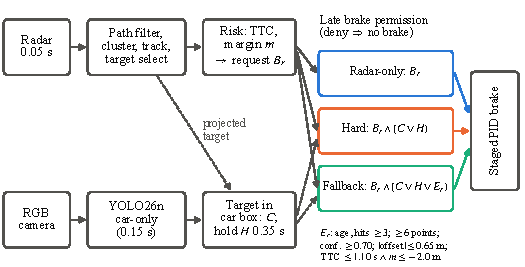
\includegraphics[width=\textwidth]{pipeline_permission_policies.pdf}
\caption{Chuỗi xử lý dùng chung từ cảm biến đến phanh. Mọi chính sách nhận cùng
một yêu cầu phanh radar $B_r$ và cùng xác nhận chỉ-ô-tô $C$/giữ xác nhận $H$,
và chỉ khác nhau ở bước cấp quyền ở khâu cuối: cổng cứng từ chối $B_r$ khi không có
hộp ô tô tại mục tiêu được chiếu; dự phòng còn cấp quyền cho $B_r$ khi điều
kiện khẩn cấp $E_r$ thỏa mãn.}
\label{fig:pipeline}
\end{figure}

Hình~\ref{fig:pipeline} tóm tắt chuỗi xử lý dùng chung. Các điểm radar được
lọc theo khoảng cách, độ cao mặt đường và quỹ đạo dự đoán có độ cong không đổi
(constant-curvature path), được phân cụm theo vị trí/vận tốc, và được liên kết
(associate) qua các khung hình. Một vết theo dõi đã được xác nhận, không cũ
(non-stale) và có liên quan đến va chạm được chọn. Với khoảng cách $d$, vận tốc
tương đối đo bởi radar $v_r<0$ và tốc độ xe chủ $v_e$,
\begin{equation}
v_c=-v_r,\qquad \mathrm{TTC}=d/v_c,\qquad v_t=\max(0,v_e+v_r).
\end{equation}
Khoảng cách dừng cần thiết và biên (margin) là
\begin{equation}
d_{\rm req}=\max\!\left(d_0,v_et_r+\frac{v_e^2}{2a_e}-\frac{v_t^2}{2a_t}+d_0\right),
\quad m=d-d_{\rm req},
\end{equation}
trong đó $t_r=0.20$ s, $a_e=8$, $a_t=6$ m/s$^2$ và $d_0=1$ m là các tham số
rủi ro danh định của mô phỏng. Các giá trị giảm tốc cực đại (peak deceleration) trình bày ở phần
sau là kết quả vòng kín (closed-loop) được ghi lại, không phải các ràng buộc
do $a_e$ áp đặt. Một bộ điều khiển PID nhiều tầng (staged PID) dùng chung cung
cấp các lệnh phanh liên tục.

Gọi $B_r$ là yêu cầu AEB từ radar, $C$ là xác nhận camera hiện tại, $H$ là xác
nhận đang được giữ, và $E_r$ là điều kiện khẩn cấp, bao gồm cả cơ chế chốt
(latch) của nó. Các chính sách cấp quyền là
\begin{align}
 B_{\rm radar}&=B_r,\\
 B_{\rm hard}&=B_r\land(C\lor H),\\
 B_{\rm fallback}&=B_r\land(C\lor H\lor E_r).
\end{align}
Một lần chấp nhận khẩn cấp mới đòi hỏi một vết theo dõi đã xác nhận/không cũ,
tuổi (age) và chuỗi lần khớp liên tiếp (hit streak) $\geq3$, ít nhất sáu điểm,
độ tin cậy của vết $\geq0.70$, độ lệch tuyệt đối so với quỹ đạo (path offset)
$\leq0.65$ m, TTC $\leq1.10$ s \emph{và} biên $m\leq-2.0$ m. Cả điều kiện TTC
và điều kiện biên đều phải thỏa mãn. Sau
khi được chấp nhận, dự phòng được chốt cho đến khi radar rời trạng thái
\texttt{BRAKE}. Độ tin cậy của vết ở đây là điểm số của bộ theo dõi (tracker
score), không phải xác suất tồn tại vật lý đã được hiệu chuẩn.

Mọi cổng đều yêu cầu $B_r$: chỉ riêng một hộp phát hiện của camera không thể
tạo ra rủi ro động học. Vì vậy, chỉ-radar là tham chiếu không hạn chế đối với
yêu cầu dùng chung đó; dự phòng không phải là chỉ-radar, vì nó có thể giữ lại
yêu cầu đó khi không có xác nhận camera cho đến khi các điều kiện khẩn cấp
chặt chẽ hơn được thỏa mãn. Chuỗi xử lý cập nhật quỹ đạo xe chủ, các vết theo
dõi, mục tiêu, rủi ro radar, suy luận camera theo lịch, quyền phanh và chấp
hành theo đúng thứ tự đó, sau đó ghi lại trạng thái tiếp theo của trình mô
phỏng.

Với cùng một trạng thái đầu vào, các phương trình trên kéo theo
$B_{\rm hard}\leq B_{\rm fallback}\leq B_{\rm radar}$ đối với quyền phanh dạng
Boolean. Đây là một tính chất của các luật, không phải là sự bảo đảm rằng các
tập kết quả vòng kín lồng nhau: các lịch sử phanh khác nhau làm thay đổi tốc
độ, các quan sát cảm biến tiếp theo và thời điểm vượt ngưỡng. Do đó, so sánh
ghép cặp sử dụng các điều kiện được thực thi riêng biệt, không dùng phát lại
phản thực (counterfactual replay) vốn giả định các phép đo tương lai giống hệt
nhau sau những hành động phanh khác nhau.

\section{Giao thức, nhãn và phân tích}
\subsection{Thực thi đã đóng băng và các bộ kịch bản được xây dựng}
Các ngưỡng, bộ kịch bản (suite) và giao thức đã được gắn thẻ (tag) trong kho
mã nguồn (repository) tại \texttt{safe-fallback-eval-v1} trước khi chạy tập
giữ lại. Các trường hợp bất lợi được thiết kế khi đã biết luật; kết quả của
chúng không được dùng để chọn hay tinh chỉnh lại các ngưỡng của luật. Đây là
một \emph{tập giữ lại kiểm tra cơ chế bất lợi đã đóng băng} (frozen adverse
mechanism hold-out), không phải một mẫu mù (blind sample) từ một phân phối
triển khai. Các thống kê theo điều kiện định danh và mức độ nghiêm trọng là
các đại lượng được suy ra hậu kiểm (post-hoc) từ các nhật ký đã đóng băng.
Không được nhầm lẫn chúng với các kết quả mới được đăng ký trước
(pre-registered).

Chiến dịch gồm 2,461 lượt chạy trong 639 phiên CARLA cô lập. Các lần lặp của
một điều kiện định danh được thực thi trước khi chuyển sang tiến trình máy
chủ (server) mới tiếp theo. Cả hai chính sách camera đều yêu cầu
\texttt{CUDAExecutionProvider}; việc sai lệch provider hoặc lỗi suy luận là
một điểm dừng cứng về kỹ thuật (technical hard stop). Các kết quả FAIL do
thuật toán đã chạy hoàn tất vẫn được giữ làm bằng chứng; chỉ những lượt chạy
chưa hoàn tất vì lý do kỹ thuật mới đủ điều kiện để chạy lại.

Bộ lõi gồm 66 điều kiện tốc độ--khoảng cách (speed--gap) bao trùm CCRm, CCRb,
cắt vào làn (cut-in) và các giới hạn liên quan, 29 kiểm thử hồi quy
(regression) hỗn hợp giữa phương tiện/trường hợp âm tính, tám vật thể tĩnh ở
mép bên (lateral edge prop), và hai mối nguy hộp/thùng phuy (box/barrel) ở
giữa đường đi: tổng cộng 105 điều kiện. Sáu điều kiện lỗi tổng hợp yếu bốn
điểm được đánh giá riêng, không được đưa vào ma trận nhầm lẫn (confusion)
chính của bộ lõi. Hai mươi nhiễu loạn (perturbation) cục bộ thay đổi tốc độ $\pm2$ km/h,
khoảng cách $\pm1$ m, thời điểm cắt vào làn $\pm0.1$ s, hoặc độ lệch của vật
thể tĩnh $\pm0.15$ m. Mười điều kiện tắt bộ phát hiện loại bỏ các phát hiện
của camera; điều này mô hình hóa việc mất phát hiện hoàn toàn chứ không phải
một phân phối thời tiết tự nhiên.

Tập giữ lại bất lợi 14 điều kiện gồm ba vật thể tĩnh mới ở giữa đường đi, bốn
kiểu ngoại hình phương tiện, hai vật thể tĩnh ở mép, và năm cấu hình hình học
bóng ma tổng hợp tồn tại dai dẳng với 6--10 điểm được chèn. Bộ lõi và tập giữ
lại dùng năm lần lặp; bộ phát triển (development) và bộ nhiễu loạn lần lượt
dùng hai và ba lần. Hạt giống 2026 được ghi lại. Không có điều kiện định danh
nào cho kết quả PASS/FAIL lẫn lộn giữa các lần lặp: các kết quả hệ thống ở cấp
điều kiện được báo cáo đều là toàn PASS hoặc toàn FAIL. Do đó, các lượt chạy
lặp lại đo tính tất định (determinism) của chuỗi xử lý mô phỏng, không phải độ
biến thiên giữa các lượt chạy (run-to-run variability) hay các tình huống giao
thông độc lập; việc thay đổi nhiễu cảm biến và hạt giống là công việc tương
lai.

\subsection{Dự đoán phanh, thành công của hệ thống và mức độ nghiêm trọng}
Các tệp YAML đã đóng băng cung cấp nhãn kỳ vọng về phanh/va chạm. Một dự đoán
phanh nghĩa là có ít nhất một tick được ghi với \texttt{aeb\_override=true};
một va chạm nghĩa là có bất kỳ tick nào với \texttt{collision\_count>0}. PASS
ở cấp hệ thống đòi hỏi kỳ vọng về phanh và va chạm đều khớp. Các trường hợp
dương tính không va chạm còn đòi hỏi khoảng cách giữa hai cản xe (bumper gap)
tối thiểu $\geq0.5$ m, kèm các khẳng định bổ sung về làn/mục tiêu khi được chỉ
định. Như vậy, một TP về phanh vẫn có thể va chạm hoặc vi phạm tiêu chí khoảng
cách dừng.

Chúng tôi báo cáo TP/FP/TN/FN, độ chính xác/độ phủ, PASS hệ thống và số lần
va chạm theo từng điều kiện định danh. Các ma trận ghép cặp đối sánh theo đúng
các mã định danh điều kiện giống nhau. Khoảng Wilson \cite{wilson1927} là các
khoảng tham chiếu nhị thức mang tính mô tả, được tính từ số đếm theo điều kiện
định danh, không phải bảo đảm về xác suất bao phủ (coverage) hay suy luận cho
tổng thể giao thông trên đường đối với lưới không ngẫu nhiên này. Các cặp
chính sách được so sánh bằng kiểm định McNemar chính xác hai phía
\cite{mcnemar1947} trên các điều kiện định danh bất đồng (discordant), được
báo cáo kèm số lượng bất đồng; kiểm định có điều kiện này mang tính bảo thủ
(conservative) khi số đếm nhỏ \cite{fagerland2013mcnemar}. Các giá trị $p$ của
nó mô tả mức độ lệch về một phía của sự bất đồng trên lưới này, không có hiệu
chỉnh đa so sánh (multiplicity adjustment) và không suy luận cho tổng thể giao
thông. Không kiểm định ý nghĩa thống kê nào coi các lần lặp là độc lập. Tỷ lệ
giữa các lớp được thiết kế có ảnh hưởng đến độ chính xác, và mẫu số nhỏ của
tập giữ lại hạn chế việc diễn giải.

Các nhãn liên quan đến nhu cầu phanh theo thiết kế trong mỗi điều kiện được
xây dựng, không phải việc YOLO có dự đoán ra lớp \emph{car} hay không. Vì vậy,
một vật thể tĩnh không phải phương tiện ở giữa đường đi là một mối nguy dương
tính ngay cả khi nó không có trong không gian nhãn (label space) của bộ phát
hiện; một bóng ma tổng hợp không có mối nguy vật lý là âm tính dù có vết theo
dõi radar ổn định. Các nhãn này cho phép đánh giá riêng rẽ việc loại bỏ theo
ngữ nghĩa (semantic rejection) và mức liên quan của mối nguy vật lý. Việc tổng
hợp theo điều kiện định danh cũng giữ được sự phân biệt giữa các thất bại:
khoảng trống không đủ (insufficient clearance), không phanh và va chạm không
thể thay thế cho nhau, và tỷ lệ PASS giống nhau không nhất thiết hàm ý thời
điểm phanh giống nhau.

Tốc độ trước va chạm (pre-impact speed) là tốc độ xe chủ được ghi lại cuối
cùng trước lần va chạm đầu tiên, một đại lượng thay thế (proxy) theo bước
0.05 s chứ không phải tốc độ tiếp xúc chính xác. Thời lượng phanh nhầm được
tính bằng số tick ghi đè (override); giảm tốc cực đại loại trừ các tick khởi
tạo, các tick dưới 1 km/h và các tick va chạm. Chúng tôi cũng báo cáo tốc
độ/khoảng cách tại thời điểm bắt đầu phanh (brake onset) và việc xe chủ có dừng xuống dưới
1 km/h hay không. Các giá trị trung vị qua các lần lặp tóm tắt quá trình thực
thi, không phải mức độ nghiêm trọng ở cấp tổng thể. Do không có mô hình người
ngồi trong xe hay mô hình xe chạy phía sau, đây là các đại lượng mô tả động
học, không phải ước lượng rủi ro chấn thương hay va chạm thứ cấp.

\section{Kết quả: lợi ích, phản ví dụ và mức độ nghiêm trọng}
\subsection{Các điểm vận hành ghép cặp}
Bảng~\ref{tab:primary} trình bày kết quả trên bộ lõi và tập giữ lại. Trên bộ
lõi, dự phòng đạt 101/105 điều kiện, so với 99 của cổng cứng và 93 của
chỉ-radar. Cả hai chính sách camera đều triệt tiêu tám trường hợp phanh nhầm
do vật thể tĩnh ở mép (bốn loại vật thể tĩnh tại hai độ lệch ngang). Chỉ-radar
và dự phòng đều phanh trước cả hai mối nguy hộp/thùng phuy ở giữa đường đi;
cổng cứng phủ quyết chúng, dẫn đến thêm hai điều kiện FN/va chạm. Mọi chính
sách đều có chung một FN trong một tình huống cắt ra khỏi làn muộn (late
cut-out), trong đó các tín hiệu phản hồi radar rời khỏi hành lang quỹ đạo dự
đoán (predicted-path corridor) $\pm$1.25 m trước khi đạt ngưỡng phanh, mặc dù
nhãn vẫn yêu cầu phanh. Các chính sách cũng có chung ba điều kiện va chạm ở tốc
độ cao. Do
đó, số điều kiện va chạm trên bộ lõi là 3/5/3 theo từng chính sách, tương ứng
15/25/15 lượt chạy lặp lại.

\begin{table}[t]
\caption{Kết quả chính theo điều kiện định danh. Các khoảng trong ngoặc vuông
là khoảng Wilson mang tính mô tả, chỉ trên lưới được xây dựng; VC: số điều
kiện va chạm.}
\label{tab:primary}
\centering\footnotesize
\setlength{\tabcolsep}{2pt}
\begin{tabular*}{\textwidth}{@{\extracolsep{\fill}}llrrrrrccrr}
\toprule Phạm vi & Chính sách & N & TP & FP & TN & FN & Độ chính xác [khoảng] & Độ phủ [khoảng] & PASS & VC\\
\midrule
Lõi & Radar & 105 & 84 & 8 & 12 & 1 & .913 [.838,.955] & .988 [.936,.998] & 93 & 3\\
 & Cứng & 105 & 82 & 0 & 20 & 3 & 1.000 [.955,1] & .965 [.901,.988] & 99 & 5\\
 & Dự phòng & 105 & 84 & 0 & 20 & 1 & 1.000 [.956,1] & .988 [.936,.998] & 101 & 3\\
\midrule
Giữ lại & Radar & 14 & 6 & 5 & 2 & 1 & .545 [.280,.787] & .857 [.487,.974] & 6 & 3\\
 & Cứng & 14 & 5 & 0 & 7 & 2 & 1.000 [.566,1] & .714 [.359,.918] & 11 & 3\\
 & Dự phòng & 14 & 6 & 4 & 3 & 1 & .600 [.313,.832] & .857 [.487,.974] & 7 & 3\\
\bottomrule
\end{tabular*}
\end{table}

Bảng~\ref{tab:paired} làm lộ ra những thay đổi bị che khuất bởi các tỷ lệ tổng
hợp. Trên bộ lõi, so với chỉ-radar, cổng cứng được thêm tám điều kiện nhưng
mất hai; dự phòng giữ được cả hai trường hợp khôi phục. Trên tập giữ lại, cổng
cứng được thêm bốn điều kiện so với dự phòng và không mất điều kiện nào xét
theo PASS hệ thống nhị phân. Với tối đa mười điều kiện bất đồng mỗi cặp, các
phép so sánh này nên được đọc thông qua số đếm của chúng
(Mục~\ref{sec:limits}). Cả ba chính sách
vẫn va chạm với ba vật thể tĩnh ở giữa đường đi. Điều này không có nghĩa là
mức giảm nhẹ va chạm (mitigation) như nhau, như mức độ nghiêm trọng của trường
hợp ghế băng dưới đây cho thấy.

\begin{table}[t]
\caption{Kết quả hệ thống ghép cặp theo điều kiện định danh. Các cột chỉ hai
chính sách A và B, không phải TP/FP về phanh; $p$: kiểm định McNemar chính xác
hai phía trên các điều kiện chỉ-A so với chỉ-B (mang tính mô tả, lưới được xây
dựng).}
\label{tab:paired}
\centering\small
\setlength{\tabcolsep}{4pt}
\begin{tabular*}{\textwidth}{@{\extracolsep{\fill}}llrrrrr}
\toprule Phạm vi & A / B & Cả hai PASS & Chỉ A & Chỉ B & Cả hai FAIL & $p$\\ \midrule
Lõi & Radar / Cứng & 91 & 2 & 8 & 4 & 0.1094\\
 & Radar / Dự phòng & 93 & 0 & 8 & 4 & 0.0078\\
 & Cứng / Dự phòng & 99 & 0 & 2 & 4 & 0.5000\\
Giữ lại & Radar / Cứng & 6 & 0 & 5 & 3 & 0.0625\\
 & Radar / Dự phòng & 6 & 0 & 1 & 7 & 1.0000\\
 & Cứng / Dự phòng & 7 & 4 & 0 & 3 & 0.1250\\
\bottomrule
\end{tabular*}
\end{table}

Cả sáu điều kiện lỗi yếu bốn điểm được đánh giá riêng đều kích hoạt phanh nhầm
ở chỉ-radar và bị cả hai chính sách camera chặn lại. Ngược lại, dự phòng chấp
nhận bốn trong năm bóng ma có mức hỗ trợ cao (high-support) của tập giữ lại,
chỉ chặn điều kiện có độ lệch 0.75 m. Các điều kiện ngoại hình phương tiện
không phân biệt được cổng cứng với dự phòng vì chúng vẫn nằm trong không gian
nhãn của camera. Thứ tự xếp hạng các chính sách thay đổi theo các cơ chế có
mặt trong bộ kịch bản, chứ không đơn thuần theo số lần thực thi lặp lại.

\subsection{Các cơ chế ở những khâu khác nhau của chuỗi xử lý}
\begin{figure}[t]
\centering
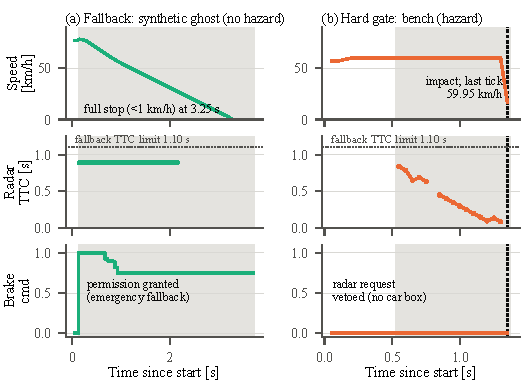
\includegraphics[width=\textwidth]{timeseries_ghost_vs_bench.pdf}
\caption{Nhật ký theo tick đã đóng băng. (a) Dự phòng, bóng ma tổng hợp sáu
điểm: cấp quyền khẩn cấp tại 0.15~s và dừng hẳn. (b) Cổng cứng, ghế băng trong
tập giữ lại: yêu cầu của radar bị phủ quyết cho đến lúc va chạm (nét đứt). Màu
xám: có yêu cầu radar $B_r$. Cách chọn: lượt chạy có các đại lượng mô tả mức độ
nghiêm trọng bằng trung vị của chính sách (tốc độ bắt đầu phanh, thời lượng và
giảm tốc cực đại của bóng ma trên 20 lượt chạy; tốc độ trước va chạm của ghế
băng trên năm lượt chạy), chọn mã kịch bản/lượt chạy nhỏ nhất khi bằng nhau.}
\label{fig:timeseries}
\end{figure}

\emph{Thiếu vết theo dõi.} Với xe đẩy mua hàng (shopping cart) trong tập giữ
lại, mỗi khung hình chỉ có tối đa hai điểm radar vượt qua bộ lọc khoảng cách,
độ cao và quỹ đạo dự đoán, và không có cụm nào được hình thành. Không có yêu cầu
phanh radar nào đến được bất kỳ cổng nào; một cơ chế ghi đè quyền phanh ở khâu
phía sau (downstream) không thể khôi phục thất bại ở thượng nguồn này. Mọi chính sách đều va chạm mà không phanh, với tốc độ thay thế
(proxy) trung vị 49.96 km/h.

\emph{Phủ quyết ngữ nghĩa và cấp quyền bị trễ (delayed permission).} Ghế băng tạo ra một vết theo dõi
radar, nhưng không có xác nhận ô tô nào dùng được
(Hình~\ref{fig:timeseries}b). Chỉ-radar phanh ở khoảng cách 12.624 m; dự phòng
đạt điều kiện ở 4.295 m; cổng cứng không phanh. Bảng~\ref{tab:severity} ghi
nhận tốc độ trước va chạm lần lượt là 32.57, 54.93 và 59.95 km/h. Dự phòng
khôi phục được một TP về phanh, chứ không phải việc dừng xe kịp thời. So với
cổng cứng, chỉ-radar làm giảm đại lượng thay thế này khoảng 27.4 km/h, trong
khi dự phòng chỉ giảm 5.0 km/h.

\emph{Va chạm dù đã được cấp quyền.} Với vật thể tĩnh cảnh báo giao thông
(traffic-warning prop), mọi chính sách đều phanh ở 21.871 m, và nhật ký của
các chính sách camera cho thấy đó là do xác nhận chứ không phải do dự phòng.
Tất cả đều va chạm ở 7.82 km/h. Bản ghi xác lập rằng quyền phanh đã được cấp;
nó không tự xác định được một khiếm khuyết về động lực học tiếp xúc hay về bộ
điều khiển.

\emph{Vết theo dõi giả có sức thuyết phục.} Một lần chèn sáu điểm ở tâm đã tạo
thành vết theo dõi được xác nhận khi đến 0.15 s, với độ tin cậy 1.0, TTC
0.89 s và biên $-15.21$ m (Hình~\ref{fig:timeseries}a). Chỉ-radar và dự phòng
yêu cầu phanh khẩn cấp; cổng cứng không có xác nhận ô tô. Các bóng ma tám và mười điểm ở tâm cùng
bóng ma tám điểm lệch 0.50 m có hành vi tương tự. Dịch điểm chèn ra 0.75 m sẽ
vượt qua biên 0.65 m đã đóng băng của dự phòng nhưng không ngăn được việc phanh
ở chỉ-radar. Đây là các phản ví dụ tổng hợp đối với tính đầy đủ của luật khẩn
cấp, không phải phép đo mức độ phổ biến của bóng ma thật.

\begin{table}[t]
\caption{Mức độ nghiêm trọng trên tập giữ lại: trung vị trên năm lượt chạy cho
mỗi điều kiện vật lý; các hàng bóng ma tổng hợp 25/20 lượt chạy. Giá trị trước
va chạm là đại lượng thay thế lấy tại tick cuối.}
\label{tab:severity}
\centering\small
\setlength{\tabcolsep}{4pt}
\begin{tabular*}{\textwidth}{@{\extracolsep{\fill}}llrr}
\toprule Cơ chế & Chính sách & \begin{tabular}[b]{@{}r@{}}Bắt đầu phanh\\/ khoảng cách\end{tabular} & \begin{tabular}[b]{@{}r@{}}Kết quả mức độ\\nghiêm trọng\end{tabular}\\ \midrule
Xe đẩy & Tất cả & không phanh & 49.96 km/h trước va chạm\\
Ghế băng & Radar & 12.624 m & 32.57 km/h trước va chạm\\
 & Cứng & không phanh & 59.95 km/h trước va chạm\\
 & Dự phòng & 4.295 m & 54.93 km/h trước va chạm\\
Cảnh báo & Tất cả & 21.871 m & 7.82 km/h trước va chạm\\
\midrule
FP bóng ma & Radar (25 lượt) & 78.4 km/h & 3.60 s / 9.02 m/s$^2$\\
 & Dự phòng (20) & 78.4 km/h & 3.60 s / 9.02 m/s$^2$\\
\bottomrule
\end{tabular*}
\end{table}

Mọi lần phanh nhầm do bóng ma đều là một lần dừng xe mô phỏng xuống dưới
1 km/h, không phải một xung kéo dài một tick: cả 20 lượt chạy bóng ma dưới
chính sách dự phòng đều dừng hẳn, sau tốc độ bắt đầu phanh trung vị 78.4 km/h,
thời lượng ghi đè trung vị 3.60 s và giảm tốc cực đại trung vị 9.02 m/s$^2$
(Bảng~\ref{tab:severity}). Điều này làm cho sự suy giảm độ chính xác có ý nghĩa
về mặt vận hành trong mô phỏng; nó không định lượng rủi ro chấn thương hay rủi
ro bị đâm từ phía sau.
FN chung ở tình huống cắt ra khỏi làn muộn và các va chạm ở giới hạn dừng tốc
độ cao lại thuộc loại khác nữa: chúng không phải bằng chứng của sự phủ quyết
từ camera, vì chỉ-radar cũng thất bại ở các điều kiện đó.

\subsection{Loại bỏ thành phần, nhiễu loạn và mất phát hiện}
Trong thí nghiệm loại bỏ thành phần (ablation) trên bộ phát triển gồm 12 điều kiện (hai
lần lặp), dự phòng đầy đủ đạt 12/12. Cổng cứng và biến thể không chốt
(no-latch) đều thất bại ở hai điều kiện hộp/thùng phuy ở giữa đường đi. Bỏ
ràng buộc quỹ đạo làm phát sinh thêm ba trường hợp phanh nhầm do vật thể tĩnh
ở mép; bỏ số điểm tối thiểu làm phát sinh thêm hai trường hợp phanh nhầm do
bóng ma yếu. Bỏ điều kiện ổn định/độ tin cậy hoặc thay phép kết hợp
TTC-AND-biên bằng OR không làm thay đổi kết quả nào trên lưới tập trung này. Vì
vậy, tính cần thiết độc lập của chúng chưa được xác lập. Sáu điều kiện phân
tích độ nhạy một yếu tố (one-factor sensitivity) cho thấy một lần phanh nhầm
khi hạ số điểm và một lần bỏ sót vật thể tĩnh ở giữa đường đi khi siết chặt
điều kiện ổn định hoặc TTC. Không có tuyên bố nào về một điểm tối ưu toàn cục.

\begin{table}[t]
\caption{Kết quả mở rộng theo điều kiện định danh, không theo lượt chạy lặp
lại.}
\label{tab:extended}
\centering\small
\setlength{\tabcolsep}{4pt}
\begin{tabular*}{\textwidth}{@{\extracolsep{\fill}}llrrrrrr}
\toprule Bộ & Chính sách & PASS/N & TP & FP & TN & FN & VC\\ \midrule
Nhiễu loạn & Radar & 19/20 & 20 & 0 & 0 & 0 & 1\\
 & Cứng & 15/20 & 15 & 0 & 0 & 5 & 5\\
 & Dự phòng & 18/20 & 20 & 0 & 0 & 0 & 1\\
\midrule
Tắt camera & Cứng & 4/10 & 0 & 0 & 4 & 6 & 6\\
 & Dự phòng & 8/10 & 6 & 0 & 4 & 0 & 2\\
\bottomrule
\end{tabular*}
\end{table}

Bảng~\ref{tab:extended} phân biệt hai thất bại trong bộ nhiễu loạn: dự phòng
va chạm ở khoảng cách tới hộp 19 m, nhưng tránh được va chạm ở 21 m và dừng
lại ở 0.353 m, dưới ngưỡng PASS 0.5 m. Đồng nhất mọi FAIL với va chạm sẽ là
không chính xác. Khi tắt các phát hiện, dự phòng phanh ở cả sáu điều kiện
dương tính nhưng va chạm ở hai điều kiện. Bốn điều kiện PASS của cổng cứng đều
là trường hợp âm tính, không phải các phản ứng thành công trước mối nguy. Các
phép thăm dò cục bộ này làm lộ sự phụ thuộc vào luật, không phải độ bền vững
(robustness) trên các bản đồ, điều kiện thời tiết hay sai số cảm biến ngẫu
nhiên.

\subsection{Tính toán và khả năng tái lập}
474 phiên bắt buộc CUDA chứa 74,928 lần suy luận và không có lỗi suy luận nào.
Trung vị theo phiên của p50/p95 là 9.95/11.53 ms; giá trị trung bình có trọng
số theo số lần suy luận là 11.56 ms. Mỗi tiến trình mới có một lần khởi động
nguội (cold start) trên 150 ms; giá trị lớn nhất là 276.10 ms. Các thời gian
xử lý ONNX đo trên máy chủ này không bao gồm radar, truyền dữ liệu, điều khiển,
hiển thị và chấp hành; chúng không phải là hạn thời gian đầu-cuối (end-to-end)
của ECU.

Bản kê phiên (session manifest) ghi lại commit, hạt giống, các phiên bản CARLA,
giá trị băm (hash) của mô hình/cấu hình, provider được cấu hình/đang hoạt
động, số lần suy luận và các lỗi. Nhật ký theo tick lưu giữ mức hỗ trợ của vết
theo dõi, độ tin cậy, TTC, biên, lý do của cổng, trạng thái ghi đè và va chạm.
Khóa điểm kiểm tra (checkpoint key) là (mã định danh kịch bản, chỉ số lượt
chạy); việc khôi phục kỹ thuật không thể biến một FAIL do thuật toán thành một
lần chạy lại thành công được chọn lọc. Ma trận nhầm lẫn theo điều kiện định
danh, kết quả ghép cặp và mức độ nghiêm trọng được tái tạo từ nhật ký đã đóng
băng mà không thêm hay bớt lượt chạy nào. Việc tái cấu trúc (refactoring) kho
mã nguồn và các thay đổi của trình khởi chạy (launcher) diễn ra sau đó và
không phải là đóng góp thực nghiệm hay sự kiểm chứng mới cho các chính sách
này.

Mã nguồn, các tệp bản thảo, tổng kiểm tra (checksum) và bằng chứng dẫn xuất đã
được tuyển chọn được lập chỉ mục tại \url{https://github.com/mvhoang92/aeb} và
được lưu trữ tại \artifactdoi; bản đồ nguồn (source map) đi kèm xác định kho
lưu trữ dữ liệu thô đã đóng băng, các script dẫn xuất và chuỗi lưu vết
checksum. Các tư liệu lớn sinh ra lúc chạy (runtime artifact) và các tệp mô
hình cục bộ được tham chiếu bằng hash và chính sách đường dẫn thay vì được
nhúng vào gói bản thảo. Việc chạy lại đòi hỏi một bản cài đặt CARLA tương
thích, tư liệu mô hình cục bộ và môi trường CUDA. Các giá trị hash xác lập danh
tính của tư liệu, không xác lập hành vi giống nhau đến từng bit độc lập với
phần cứng.

\section{Thảo luận và tính hiệu lực}
\subsection{Những gì phép so sánh xác lập được}
Các kết quả định vị ba câu hỏi khác nhau: radar có hình thành được mục tiêu
không, chính sách có cho phép phanh không, và hành động được cho phép có đạt
được mức giảm nhẹ va chạm đủ hay không? Gộp chúng vào một tỷ lệ thành công duy
nhất sẽ che khuất cả việc cấp quyền dự phòng bị trễ ở trường hợp ghế băng lẫn va chạm tốc
độ thấp ở vật thể tĩnh cảnh báo. Tương tự, luật khẩn cấp cải thiện độ phủ trên
bộ lõi nhưng lại chấp nhận các bóng ma có cùng các thuộc tính đủ điều kiện.
Tính bền vững theo thời gian (persistence) của vết theo dõi và mức hỗ trợ bằng
số điểm củng cố một ước lượng mà không tự chứng minh được rằng một vật cản vật
lý thực sự tồn tại.

Đây là hạn chế của thông tin và các ngưỡng được thử nghiệm, không phải một định
lý bất khả (impossibility theorem) đối với hợp nhất radar-camera. Ở đây, cổng
cứng được ưu thế theo PASS nhị phân trên tập giữ lại, nhưng không theo mức giảm
nhẹ va chạm ở trường hợp ghế băng; dự phòng có ưu thế trên bộ lõi, nhưng các
lần phanh nhầm của nó trên tập giữ lại đều là dừng hẳn. Chúng tôi không đề
xuất một chính sách phổ quát bằng cách gán các trọng số tùy ý cho những kết
quả không tương thích này. Một phép so sánh hữu ích tiếp theo phải bao gồm xác
minh thị giác không phụ thuộc lớp (class-agnostic visual verification) và một
cổng mềm được ghép theo độ tin cậy (confidence-matched soft gate) trước khi
quy các cải thiện cho một thuật toán hợp nhất mới. Các phương pháp xác suất
đòi hỏi hiệu chuẩn và bằng chứng vượt ra ngoài một điểm số bộ theo dõi được
đổi tên \cite{sandblom2011threat,lindenmaier2022existence}.

Các câu trả lời thu được cho RQ1--RQ3 mang tính có điều kiện nhưng có thể dùng
để hành động. Các cải thiện của chính sách có thể truy về một số ít cơ chế đã
được xác định thay vì một ``cải thiện nhờ hợp nhất'' chung chung. Một cơ chế
ghi đè không thể khắc phục sự vắng mặt của một vết theo dõi ở thượng nguồn, và
việc vượt qua một ngưỡng chất lượng radar có thể vừa chấp nhận một bóng ma vừa
làm trễ việc phanh trước một vật cản thật. Cuối cùng, tránh va chạm, giảm nhẹ
va chạm và can thiệp không mong muốn là các mục tiêu riêng biệt. Một chính
sách thắng ở một mục tiêu không nên được lựa chọn dựa trên một chỉ số F1 tổng
hợp hay tỷ lệ PASS duy nhất mà không nêu rõ điều kiện vận hành dự kiến và chi
phí sai số chấp nhận được.

\subsection{Giới hạn của bằng chứng}\label{sec:limits}
Các kết luận dựa trên các cơ chế đã được xác định, không dựa trên ý nghĩa
thống kê: trên lưới được xây dựng này, chỉ một trong sáu phép so sánh McNemar
chính xác (chỉ-radar so với dự phòng trên bộ lõi, 0 so với 8, $p=0.0078$) nhỏ
hơn 0.05.
Thí nghiệm bao gồm một bản đồ, một nền tảng xe chủ, một hạt giống cố định, điều
kiện ghi hình thuận lợi và một bộ phát hiện chỉ nhận lớp ô tô trong miền. Tập giữ lại 14 điều kiện được chủ ý xây
dựng khi đã biết luật. Nó kiểm tra các cơ chế bất lợi chứ không kiểm tra khả
năng tổng quát hóa không thiên lệch. Radar mức điểm của CARLA không tái tạo đầy
đủ vật lý đa đường; chèn lỗi không ước lượng được tần suất bóng ma radar thật
\cite{kraus2021ghost,magosi2022radar}. Tick cuối trước va chạm có độ rời rạc
hóa 0.05 s, và các đại lượng động học của phanh nhầm không phải là chi phí
chấn thương. Không có khảo sát quét (sweep) nhiều bản đồ/thời tiết/hệ số ma
sát, thí nghiệm với cảm biến thật, HIL, chứng minh an toàn chức năng
(functional safety) hay chứng nhận theo tiêu chuẩn.

Cũng không có mốc so sánh được ghép tương xứng (matched) dạng cổng mềm, không
phụ thuộc lớp, dựa trên học máy hay theo xác suất. Hạn chế về phủ quyết của
camera phụ thuộc vào không gian nhãn chỉ-ô-tô đã chọn, không phải một tuyên bố
về mọi hệ thống camera. Các mốc so sánh mở rộng đòi hỏi một giao thức phát
triển/đánh giá mới; tập giữ lại đã được xem xét có thể tiếp tục là dữ liệu hồi
quy nhưng không thể tiếp tục là bằng chứng kiểm tra chưa từng thấy. Ràng buộc
này bảo toàn các kết quả bất lợi hiện tại thay vì tinh chỉnh để loại bỏ các
phản ví dụ.

\section{Kết luận}
Trong một chuỗi xử lý CARLA cố định, dự phòng khẩn cấp khôi phục hai mối nguy
trên bộ lõi bị camera phủ quyết trong khi vẫn duy trì việc triệt tiêu phanh
nhầm do vật thể tĩnh ở mép. Bốn điều kiện bóng ma tổng hợp tồn tại dai dẳng
đảo ngược lợi thế của nó so với cổng cứng trên tập giữ lại bất lợi. Các lần
phanh nhầm dừng hẳn và mức giảm nhẹ bị trễ ở trường hợp ghế băng cho thấy vì
sao chỉ riêng độ phủ phanh và số lần va chạm là không đủ. Bằng chứng ủng hộ
một phép so sánh các chính sách cấp quyền có tính đến cơ chế và mức độ nghiêm
trọng, chứ không ủng hộ một lợi thế chung của hợp nhất. Thiếu xác nhận từ
camera không phải là bằng chứng đường trống, và sự hỗ trợ ổn định từ radar
không phải là bằng chứng có mối nguy vật lý.

\bibliographystyle{IEEEtran}
\bibliography{../references}

% ---------------------------------------------------------------------------
% Phần bổ sung duy nhất so với bản tiếng Anh: bảng thuật ngữ.
\clearpage
\section*{Phụ lục: Bảng thuật ngữ Anh–Việt}
\addcontentsline{toc}{section}{Phụ lục: Bảng thuật ngữ Anh–Việt}
\begingroup\small
\setlength{\LTpre}{0.5em}
\begin{longtable}{@{}p{0.42\textwidth}p{0.54\textwidth}@{}}
\toprule
\textbf{Tiếng Anh} & \textbf{Tiếng Việt dùng trong bản dịch}\\
\midrule\endhead
\bottomrule\endfoot
ablation & loại bỏ thành phần\\
actor truth & thông tin thật của actor\\
adverse hold-out & tập giữ lại bất lợi\\
artifact / artifact trail & tư liệu / chuỗi lưu vết tư liệu\\
automatic emergency braking (AEB) & phanh khẩn cấp tự động (AEB)\\
baseline & mốc so sánh\\
Bayesian object-existence estimation & ước lượng sự tồn tại của đối tượng theo Bayes\\
bench & ghế băng\\
blind sample & mẫu mù\\
box/barrel & hộp/thùng phuy\\
brake-permission policy & chính sách cấp quyền phanh\\
bumper gap & khoảng cách giữa hai cản xe\\
calibrated existence inference & suy luận tồn tại đã được hiệu chuẩn\\
camera gating & cổng camera\\
car-only camera detector & bộ phát hiện camera chỉ nhận lớp ô tô\\
central (hazard, prop) & ở giữa đường đi\\
checkpoint key & khóa điểm kiểm tra\\
class-agnostic visual verification & xác minh thị giác không phụ thuộc lớp\\
closed-loop & vòng kín\\
closest-in-path vehicle & phương tiện gần nhất trên đường đi\\
cold start & khởi động nguội\\
confidence-matched soft gate & cổng mềm được ghép theo độ tin cậy\\
constant-curvature path & quỹ đạo có độ cong không đổi\\
core (conditions, suite) & (điều kiện, bộ) lõi\\
corner case & trường hợp biên\\
counterfactual replay & phát lại phản thực\\
cut-in / cut-out & cắt vào làn / cắt ra khỏi làn\\
delayed permission & cấp quyền bị trễ\\
determinism & tính tất định\\
discordant & bất đồng\\
downstream & khâu phía sau\\
ego (vehicle) & xe chủ\\
emergency override & cơ chế ghi đè khẩn cấp\\
emergency qualification & việc đủ điều kiện khẩn cấp\\
extrinsics & tham số ngoại\\
fail / pass (system) & FAIL / PASS (giữ nguyên); “đạt” khi dùng như động từ\\
failure severity & mức độ nghiêm trọng của thất bại\\
false braking / false brake & phanh nhầm\\
fault injection & chèn lỗi\\
fault-free perception insufficiencies & thiếu hụt về nhận thức khi không có lỗi\\
free road & đường trống\\
front-to-rear crash & va chạm đuôi\\
frozen & đã đóng băng\\
fusion / fusion primitive & hợp nhất / thành phần hợp nhất cơ sở\\
graded braking & phanh phân cấp\\
hard (car-camera) gating & cổng (camera) cứng\\
hit streak & chuỗi lần khớp liên tiếp\\
hold-out & tập kiểm tra giữ lại (gọi tắt: tập giữ lại)\\
in-domain / out-of-domain & trong miền / ngoài miền\\
information boundary & ranh giới thông tin\\
label space & không gian nhãn\\
latch / no-latch & chốt / không chốt\\
late brake-permission policy & chính sách cấp quyền phanh ở khâu cuối\\
log & nhật ký\\
margin (stopping margin) & biên (biên dừng)\\
mitigation & giảm nhẹ va chạm\\
multipath & đa đường\\
multiplicity adjustment & hiệu chỉnh đa so sánh\\
named condition & điều kiện định danh\\
non-stale / stale confirmation & không cũ / xác nhận cũ\\
onset (brake onset) & bắt đầu phanh\\
paired (outcomes) & ghép cặp (kết quả ghép cặp)\\
path offset & độ lệch so với quỹ đạo\\
peak deceleration & giảm tốc cực đại\\
perception–risk–actuation chain & chuỗi nhận thức–rủi ro–chấp hành\\
permission & cấp quyền / quyền phanh\\
perturbation & nhiễu loạn\\
post-hoc & hậu kiểm\\
post-permission stopping & dừng xe sau khi được cấp quyền\\
pre-impact speed / severity & tốc độ / mức độ nghiêm trọng trước va chạm\\
pre-registered & đăng ký trước\\
precision / recall & độ chính xác / độ phủ\\
predicted-path corridor & hành lang quỹ đạo dự đoán\\
probabilistic threat assessment & đánh giá mối đe dọa theo xác suất\\
prop (edge prop, lateral edge prop) & vật thể tĩnh (ở mép, ở mép bên)\\
proxy & đại lượng thay thế\\
radar emergency fallback & dự phòng khẩn cấp bằng radar (gọi tắt: dự phòng)\\
radar ghost / synthetic (radar) ghost & bóng ma radar / bóng ma radar tổng hợp\\
radar risk stage & khâu đánh giá rủi ro radar\\
radar-only & chỉ dùng radar (gọi tắt: chỉ-radar)\\
regression & kiểm thử hồi quy\\
robustness & độ bền vững\\
rule-directed fault injection & chèn lỗi được định hướng theo luật\\
run-to-run variability & độ biến thiên giữa các lượt chạy\\
scenario-based evaluation & đánh giá dựa trên kịch bản\\
seed & hạt giống ngẫu nhiên\\
semantic rejection & loại bỏ theo ngữ nghĩa\\
sensor-to-brake pipeline & chuỗi xử lý từ cảm biến đến phanh\\
session manifest & bản kê phiên\\
shopping cart & xe đẩy mua hàng\\
split (train/val/test) & phần chia (huấn luyện/kiểm định/kiểm tra)\\
staged PID & PID nhiều tầng\\
suite & bộ kịch bản\\
technical hard stop & điểm dừng cứng về kỹ thuật\\
track / track formation & vết theo dõi / hình thành vết theo dõi\\
tracker score & điểm số của bộ theo dõi\\
traffic-warning prop & vật thể tĩnh cảnh báo giao thông\\
type approval & phê duyệt kiểu\\
unwanted activation / intervention & kích hoạt / can thiệp không mong muốn\\
upstream & thượng nguồn (khâu phía trước)\\
veto & phủ quyết\\
\end{longtable}
\endgroup

\end{document}
